\section{Problem description}\label{sec:problem}
\subsection{Problem statement}
Consider a railway line with a set of stations and directed sections, and a set of prescribed trains, each of which must operate along its specified station sequence. The input data include the train types; the arrival and departure time windows of all events; pure running times with additional acceleration and deceleration times; maximum running time supplements; minimum, normal maximum, and waiting maximum dwell times; minimum section and station headways; the track layout of each station with its arrival--departure tracks, main tracks, and receiving and departure routes; route headways; maintenance windows; train stop-count and station service frequency requirements; maximum travel times; and preferred departure and arrival windows. The problem is to determine the stopping pattern, the arrival and departure times, the train orders on sections, and the station routings of all trains.

\Cref{fig:network} links train movements along the line to the track layouts within stations. A train operation at a station refers to the stop or pass of a train at that station. A station routing alternative combines a track with a compatible receiving route and departure route; origin and destination operations require only the departure or the receiving route, respectively. The admissible alternatives depend on the train type, direction, track restrictions, and whether the train stops at or passes through the station. Intermediate operations may be optional stops, mandatory stops, or mandatory passes, whereas origin and destination operations are stops. A stop adds dwell time and the acceleration and deceleration times on the adjacent sections, while a pass has identical arrival and departure times.

\begin{figure}[tb]
\centering
\resizebox{\textwidth}{!}{% Figure 1: macroscopic line and microscopic station layouts (TikZ)
\begin{tikzpicture}[x=1cm,y=1cm,font=\footnotesize,
  stn/.style={circle,draw=gray!70!black,fill=white,inner sep=0pt,minimum size=5pt},
  hub/.style={circle,draw=blue!60!black,fill=blue!12,inner sep=0pt,minimum size=8pt},
  sec/.style={-{Stealth[length=4pt]},gray!70!black,line width=0.5pt},
  trk/.style={gray!75,line width=0.6pt},
  sel/.style={blue!65!black,line width=1.6pt},
  sw/.style={circle,draw=gray!75,fill=white,inner sep=0pt,minimum size=2.4pt},
  tlab/.style={font=\scriptsize,inner sep=1pt,anchor=south}]
% ---------------- (a) macroscopic line
\node[anchor=west,font=\footnotesize\bfseries] at (-0.15,0.75) {(a) Macroscopic level: train movements along the line};
\foreach \n/\x in {O/0,W/2.6,Z/11.0,T/13.6}{\node[stn] (\n) at (\x,0) {}; \node[above=1pt] at (\n.north) {$\n$};}
\node[hub] (X) at (5.2,0) {}; \node[above=1pt] at (X.north) {$X$};
\node[hub] (Y) at (8.4,0) {}; \node[above=1pt] at (Y.north) {$Y$};
\draw[sec] (O)--(W); \draw[sec] (W)--(X); \draw[sec] (X)--(Y); \draw[sec] (Y)--(Z); \draw[sec] (Z)--(T);
\node[tlab] at (1.3,0.03) {Running times};
\node[tlab] at (6.8,0.03) {Headways and train orders};
\node[tlab] at (12.3,0.03) {Stopping patterns};
% ---------------- station boxes and links
\draw[rounded corners=3pt,draw=gray!60,fill=gray!4] (0,-1.15) rectangle (6.55,-4.85);
\draw[rounded corners=3pt,draw=gray!60,fill=gray!4] (7.05,-1.15) rectangle (13.6,-4.85);
\draw[dashed,blue!60!black] (X.south west)--(0,-1.15); \draw[dashed,blue!60!black] (X.south east)--(6.55,-1.15);
\draw[dashed,blue!60!black] (Y.south west)--(7.05,-1.15); \draw[dashed,blue!60!black] (Y.south east)--(13.6,-1.15);
\node[fill=white,inner sep=1pt,text=blue!60!black,font=\scriptsize] at (2.0,-0.62) {Shared arrival/departure times and stop plans};
\node[fill=white,inner sep=1pt,text=blue!60!black,font=\scriptsize] at (11.6,-0.62) {Shared arrival/departure times and stop plans};
\node[anchor=west,font=\footnotesize\bfseries] at (0.1,-1.42) {(b) Microscopic level: station $X$};
\node[anchor=west,font=\footnotesize\bfseries] at (7.15,-1.42) {(c) Microscopic level: station $Y$};
% ---------------- generic station drawing: #1 x-shift, list of track y/labels, selected track y
\foreach \sx/\tracks/\ysel in {
   0/{-2.15/Track 1,-2.95/Track 3 (main track),-3.75/Track 2},
   7.05/{-1.9/Track 1,-2.425/Track 2,-2.95/Track 3 (main track),-3.475/Track 4,-4.0/Track 5}}{
 \begin{scope}[shift={(\sx,0)}]
  \def\ym{-2.95}
  \foreach \y/\lab in \tracks {
    \draw[trk] (1.35,\ym)--(1.95,\y)--(4.55,\y)--(5.15,\ym);
    \node[sw] at (1.95,\y) {}; \node[sw] at (4.55,\y) {};
    \node[tlab] at (3.25,\y) {\lab};}
  \draw[trk] (0.25,\ym)--(1.35,\ym); \draw[trk] (5.15,\ym)--(6.3,\ym);
  \node[anchor=west,font=\scriptsize] at (0.1,-4.3) {Entry throat area};
  \node[anchor=east,font=\scriptsize] at (6.45,-4.3) {Exit throat area};
  \node[text=blue!65!black,font=\scriptsize] at (3.27,-4.62) {Receiving route + arrival--departure track + departure route};
 \end{scope}}
% selected alternatives
\draw[sel] (0.25,-2.95)--(1.35,-2.95)--(1.95,-3.75)--(4.55,-3.75)--(5.15,-2.95)--(6.0,-2.95);
\draw[sel,-{Stealth[length=6pt]}] (5.9,-2.95)--(6.3,-2.95);
\draw[sel] (7.3,-2.95)--(8.4,-2.95)--(9.0,-2.425)--(11.6,-2.425)--(12.2,-2.95)--(13.05,-2.95);
\draw[sel,-{Stealth[length=6pt]}] (12.95,-2.95)--(13.35,-2.95);
\node[tlab,text=blue!65!black,fill=gray!4] at (3.25,-3.75) {Track 2};
\node[tlab,text=blue!65!black,fill=gray!4] at (10.3,-2.425) {Track 2};
% ---------------- legend
\draw[sel] (0.3,-5.25)--(1.1,-5.25); \node[anchor=west] at (1.2,-5.25) {Selected station routing alternative};
\draw[trk] (7.35,-5.25)--(8.15,-5.25); \node[anchor=west] at (8.25,-5.25) {Other station routing alternatives};
\end{tikzpicture}
}
\caption{Illustrative railway line and station track layouts. Blue paths mark the selected station routing alternatives, which are linked to the line by shared arrival and departure times and stop plans.}\label{fig:network}
\end{figure}

A feasible timetable satisfies two levels of constraints. At the macroscopic level, it satisfies the arrival and departure time windows, running and dwell times, minimum headways, train orders, overtaking rules, maintenance windows, maximum travel times, and service frequency requirements. Train stop-count constraints bound the number of stops of a train over a designated route segment, and station service frequency constraints bound the number of stopping trains of a given type at a station within a given service-counting window. A change in arrival or departure time can therefore alter the counted service even if the stopping pattern remains unchanged. At the microscopic level, every train operation is assigned a station routing alternative such that track occupations do not overlap and route headways are respected. The timetable is jointly feasible, i.e., conflict-free at both levels, if both levels are satisfied by the same arrival and departure times, stopping patterns, and station routings.

The objective is lexicographic. The primary objective minimizes the timetable makespan, i.e., the time between the earliest origin departure and the latest destination arrival over all trains. Minimizing the makespan compresses the prescribed services into the shortest operating period while respecting the service frequency requirements and travel time limits. The secondary objectives minimize the weighted deviation from preferred departure and arrival windows and, finally, the total running time supplement.

\subsection{Event-activity network representation}\label{sec:ean}
We represent the problem on an event-activity network, extending the event-based representation of timetables \citep{Serafini1989,Liebchen2007} with the disjunctive activities used for scheduling with shared resources \citep{Bartusch1988,Mascis2002}. Each node is an \emph{event}: the departure of a train at its origin, its arrival at its destination, or its arrival or departure at an intermediate station. Two virtual events $T^-$ and $T^+$ mark the start and the end of the operating period, and a time-origin event $o$ with $t_o=0$ carries absolute time bounds. Each arc $(e,f)$ is an \emph{activity} with a lower bound $l_{ef}$ on its duration, i.e., $t_f-t_e\ge l_{ef}$; an upper bound $t_f-t_e\le u_{ef}$ is represented by the reverse arc $(f,e)$ with $l_{fe}=-u_{ef}$. The activity types are as follows.
\begin{itemize}
\item \emph{Running activities} link the departure at one station with the arrival at the next station of the same train. Their duration lies between the pure running time plus acceleration and deceleration times, which depend on whether the train stops at the two stations, and the same value plus the maximum running time supplement.
\item \emph{Dwell activities} link the arrival and the departure of an intermediate operation. Their duration is zero for a pass; for a stop, it lies between the minimum dwell time and the normal maximum, or the waiting maximum if the train is overtaken.
\item \emph{Section headway activities} link the departures (and the arrivals) of two trains that use the same directed section. They form disjunctive pairs, one for each possible train order; the same order is selected at both ends of a section, so that overtaking can only take place at stations. The minimum headway depends on whether each train stops or passes.
\item \emph{Track occupation activities} link the end of the occupation of one operation with the start of the occupation of another operation at the same station. They exist only if both operations select the same track, and they form a disjunctive pair.
\item \emph{Route headway activities} link the arrival or departure events of two trains at the same station whose selected routes are subject to a route headway. They exist only if the corresponding routes are selected, and they also form disjunctive pairs.
\item \emph{Window activities} link the time origin $o$ with events and represent the arrival and departure time windows, the maintenance windows (traversal before or after the closure), and the position of a stop relative to a service-counting window (before, within, or after it).
\item \emph{Travel time activities} bound the time between the start and the end of a designated journey of a train, and \emph{makespan activities} link $T^-$ with every origin departure and every destination arrival with $T^+$.
\end{itemize}

\Cref{fig:ean}(a) shows the network for two trains $i$ and $j$ running from station $v_1$ to $v_3$ via $v_2$. The running and dwell activities of each train form a chain; the section headway pairs (blue) and the track occupation and route headway pairs at $v_2$ (orange) are disjunctive, and the latter are conditional on the station routing decisions. The discrete decisions of the problem therefore determine \emph{which} activities exist and \emph{how long} they are: the stopping decisions determine the running and dwell bounds and the minimum headways; the train orders select one activity of each section headway pair; the station routings activate track occupation and route headway pairs, of which the orders select one; and the window classifications select one window activity per counted stop. \Cref{fig:ean}(b) shows the network after such a selection, in which train $j$ overtakes train $i$ at $v_2$ while $i$ dwells longer. Once a selection is made, the event times only need to satisfy the remaining difference constraints, and the timetable makespan is determined by the longest chain of tight activities from $T^-$ to $T^+$ (\cref{prop:longest}).

\begin{figure}[tbp]
\centering
\resizebox{\textwidth}{!}{% Event-activity network of two trains i, j on stations v1 -> v2 -> v3 (TikZ)
\newcommand{\eanbase}[1]{%
  % #1 = 1: full network; 2: selected network with critical path
  \begin{tikzpicture}[x=1cm,y=1cm,font=\footnotesize,
    ev/.style={circle,draw=black!80,fill=white,inner sep=0pt,minimum size=17pt,font=\scriptsize},
    vv/.style={rectangle,rounded corners=2pt,draw=black!70,fill=gray!12,inner sep=2pt,minimum size=14pt,font=\scriptsize},
    run/.style={-{Stealth[length=4pt]},line width=0.7pt,black!80},
    dwl/.style={-{Stealth[length=4pt]},line width=0.7pt,black!80,densely dashdotted},
    hw/.style={{Stealth[length=4pt]}-{Stealth[length=4pt]},line width=0.6pt,blue!65!black,dashed},
    hws/.style={-{Stealth[length=4pt]},line width=0.7pt,blue!65!black},
    stn/.style={{Stealth[length=4pt]}-{Stealth[length=4pt]},line width=0.6pt,orange!80!black,dotted},
    stns/.style={-{Stealth[length=4pt]},line width=0.7pt,orange!80!black},
    vir/.style={-{Stealth[length=4pt]},line width=0.5pt,gray},
    crit/.style={line width=2.2pt,red!70!black,opacity=0.35}]
    % station columns
    \foreach \x/\lab in {0/$v_1$,3.6/$v_2$,7.2/$v_3$}{\node[font=\footnotesize\bfseries,gray] at (\x+0.6,3.05) {\lab};}
    \draw[gray!40,rounded corners=3pt] (2.95,-0.55) rectangle (5.45,2.5);
    \node[gray,font=\scriptsize,anchor=north] at (4.2,-0.55) {station $v_2$ (overtaking allowed)};
    % events
    \node[ev] (di1) at (0.6,2) {$d_i^{1}$};  \node[ev] (dj1) at (0.6,0) {$d_j^{1}$};
    \node[ev] (ai2) at (3.4,2) {$a_i^{2}$};  \node[ev] (aj2) at (3.4,0) {$a_j^{2}$};
    \node[ev] (di2) at (5.0,2) {$d_i^{2}$};  \node[ev] (dj2) at (5.0,0) {$d_j^{2}$};
    \node[ev] (ai3) at (7.8,2) {$a_i^{3}$};  \node[ev] (aj3) at (7.8,0) {$a_j^{3}$};
    \node[vv] (Tm) at (-1.3,1) {$T^-$}; \node[vv] (Tp) at (9.7,1) {$T^+$};
    \node[gray,font=\scriptsize,anchor=east] at (-0.15,2) {train $i$};
    \node[gray,font=\scriptsize,anchor=east] at (-0.15,0) {train $j$};
    \ifnum#1=1
      % train activities
      \draw[run] (di1)--node[above,font=\scriptsize]{running} (ai2); \draw[dwl] (ai2)--node[above,font=\scriptsize]{dwell} (di2); \draw[run] (di2)--node[above,font=\scriptsize]{running} (ai3);
      \draw[run] (dj1)--(aj2); \draw[dwl] (aj2)--(dj2); \draw[run] (dj2)--(aj3);
      % disjunctive headway pairs (one order variable per section)
      \draw[hw] (di1)--node[left,font=\scriptsize,blue!65!black]{$z_{ijc_1}$} (dj1);
      \draw[hw] (ai2) to[bend right=18] node[left,font=\scriptsize,blue!65!black,pos=0.3]{$z_{ijc_1}$} (aj2);
      \draw[hw] (di2) to[bend left=18] node[right,font=\scriptsize,blue!65!black,pos=0.3]{$z_{ijc_2}$} (dj2);
      \draw[hw] (ai3)--node[right,font=\scriptsize,blue!65!black]{$z_{ijc_2}$} (aj3);
      % conditional station activities at v2 (track occupancy / route headway)
      \draw[stn] (di2) to[bend left=6] (aj2);
      \draw[stn] (dj2) to[bend left=6] (ai2);
      \node[orange!80!black,font=\scriptsize,align=center,fill=white,inner sep=1pt] at (4.2,1.0) {$w^T,w^{\sigma\sigma'}$\\[-1pt]$\mid Y$};
      % virtual makespan events
      \foreach \e in {di1,dj1}{\draw[vir] (Tm)--(\e);}
      \foreach \e in {ai3,aj3}{\draw[vir] (\e)--(Tp);}
    \else
      % selected network: i first on c1; j overtakes i at v2 (j first on c2); different tracks, route headway active
      \draw[crit] (Tm.east)--(di1.west); \draw[crit] (di1)--(dj1); \draw[crit] (dj1)--(aj2); \draw[crit] (aj2)--(dj2);
      \draw[crit] (dj2)--(di2); \draw[crit] (di2)--(ai3); \draw[crit] (ai3.east)--(Tp.west);
      \draw[run] (di1)--(ai2); \draw[dwl] (ai2)--(di2); \draw[run] (di2)--(ai3);
      \node[font=\scriptsize,anchor=south] at (4.2,2.04) {$\eta_i=1$};
      \draw[run] (dj1)--(aj2); \draw[dwl] (aj2)--(dj2); \draw[run] (dj2)--(aj3);
      \draw[hws] (di1)--node[left,font=\scriptsize,blue!65!black]{$h$} (dj1);
      \draw[hws] (ai2) to[bend right=18] (aj2);
      \draw[hws] (dj2) to[bend right=18] node[right,font=\scriptsize,blue!65!black,pos=0.6]{$h$} (di2);
      \draw[hws] (aj3)--(ai3);
      \draw[stns] (ai2) to[bend left=10] (aj2.north east);
      \node[font=\scriptsize,text=orange!80!black,anchor=west] at (3.75,1.0) {$h_{\rho\rho'}$};
      \foreach \e in {di1,dj1}{\draw[vir] (Tm)--(\e);}
      \foreach \e in {ai3,aj3}{\draw[vir] (\e)--(Tp);}
      \node[red!70!black,font=\scriptsize,anchor=north] at (4.2,-0.95) {critical path: length $=S$ (Proposition~\ref{prop:longest})};
    \fi
  \end{tikzpicture}}
\begin{tikzpicture}[font=\footnotesize]
  \node (a) at (0,0) {\eanbase{1}};
  \node[anchor=north] (b) at ([yshift=-4mm]a.south) {\eanbase{2}};
  \node[anchor=south west,font=\footnotesize\bfseries] at (a.north west) {(a) Event-activity network with disjunctive and conditional activities};
  \node[anchor=south west,font=\footnotesize\bfseries] at (b.north west) {(b) Network after selecting stops, orders, and station routings};
  % legend
  \matrix[anchor=north,below=3mm of b,column sep=3mm,row sep=1mm,font=\scriptsize,
          nodes={anchor=west}] {
    \draw[-{Stealth[length=4pt]},line width=0.7pt] (0,0)--(0.6,0); & \node{running activity}; &
    \draw[-{Stealth[length=4pt]},line width=0.7pt,densely dashdotted] (0,0)--(0.6,0); & \node{dwell activity}; &
    \draw[{Stealth[length=4pt]}-{Stealth[length=4pt]},line width=0.6pt,blue!65!black,dashed] (0,0)--(0.6,0); & \node{section headway pair (order $z$)}; \\
    \draw[{Stealth[length=4pt]}-{Stealth[length=4pt]},line width=0.6pt,orange!80!black,dotted] (0,0)--(0.6,0); & \node{track/route activity (if selected)}; &
    \draw[-{Stealth[length=4pt]},line width=0.5pt,gray] (0,0)--(0.6,0); & \node{makespan activity}; &
    \draw[line width=2.2pt,red!70!black,opacity=0.35] (0,0)--(0.6,0); & \node{critical (tight) activities}; \\
  };
\end{tikzpicture}
}
\caption{Event-activity network for two trains $i$ and $j$ travelling from $v_1$ to $v_3$. (a) Running and dwell activities form one chain per train; section headway pairs are selected by the train order $z$ (one order per section), and track occupation and route headway pairs exist only for the selected station routings $Y$. (b) After the selection ($i$ before $j$ on $c_1$; $j$ overtakes $i$ at $v_2$; different tracks with an active route headway), the shaded critical path determines the timetable makespan.}\label{fig:ean}
\end{figure}

The representation is used in three ways. First, the mathematical formulation in \cref{sec:model} is organized by activity type, so that every constraint corresponds to one type of arc in \cref{fig:ean}. Second, the conflicts diagnosed by the algorithm are violated activities: macroscopic conflicts are violated running, dwell, section headway, window, or travel time activities, and station conflicts are violated track occupation or route headway activities. Third, for a fixed selection, the activities with zero slack identify the decisions that must change to reduce the makespan; the quality search of the algorithm builds its neighborhoods from these activities (\cref{sec:joint}).

\subsection{Interdependence of stop planning, timetabling, and platforming}
\Cref{fig:exchange} illustrates how a coordinated stop exchange can resolve a track conflict at station $X$ while maintaining the service frequencies. Train $B$ cannot stop at $X$ without overlapping the occupations of trains $A$ and $C$, and the main track cannot accommodate a stop. Exchanging the stops of trains $B$ and $D$ between stations $X$ and $Y$ preserves the displayed train and station counts, but the revised times and station routings still require feasibility checks. Even if a stop is retained, moving its reference event across a service-counting window boundary can change the station count. A compensating stop on another train must respect its stop-count limits, other service frequency requirements, and station track and route constraints. On the event-activity network, the exchange removes the dwell and track occupation activities of $B$ at $X$, adds those of $D$, changes the running activities and minimum headways of both trains, and may change the selected window activities. These dependencies require coordinated changes to stops, arrival and departure times, and station routings, with affected counts remaining within their prescribed bounds.

\begin{figure}[tb]
\centering
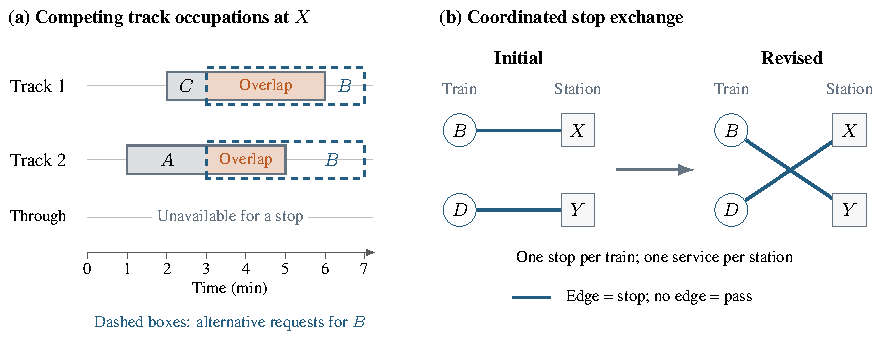
\includegraphics[width=0.85\textwidth]{figures/fig2_stop_exchange.pdf}
\caption{Illustrative stop exchange: (a) competing track occupations at station $X$; (b) revised stops preserving the displayed train and station service frequencies.}\label{fig:exchange}
\end{figure}

\subsection{Assumptions}
The following assumptions are made throughout the paper.
\begin{enumerate}[label=(A\arabic*)]
\item The train services, their station sequences, and their train types are prescribed, and no train can be cancelled. Rolling stock circulation, passenger assignment, and infrastructure changes are not considered.
\item Train operations in the two directions do not interfere with each other. Overtaking is only possible at stations where it is allowed, and a stopping train can be overtaken by at most one other train at a station. A dwell time longer than the normal maximum is permitted only for such waiting and is subject to a separate upper bound.
\item The timetable is non-periodic and covers one operating day, with arrival and departure times on a continuous time scale.
\item An intermediate stop occupies its track from arrival to departure, whereas a pass and the departure (arrival) at an origin (destination) occupy the track only at the instant of departure (arrival); no additional time is reserved for train preparation or stabling. The separation between movements of different trains in a station is represented by route headways.
\item Maintenance windows are given; each window closes a directed section during a fixed period.
\end{enumerate}
